% ex: ts=2 sw=2 sts=2 et filetype=tex
% SPDX-License-Identifier: CC-BY-SA-4.0

\clearpage
\question Usa la siguiente cuadricula para resolver los siguientes incisos:

  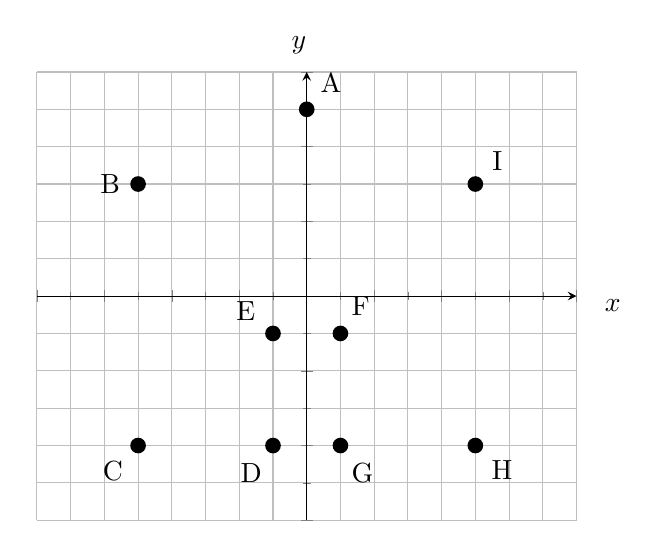
\begin{tikzpicture}
    \begin{axis}[grid=both,ymin=-6,ymax=6,xmax=8,xmin=-8,xticklabel=\empty,yticklabel=\empty,
               minor tick num=1,axis lines = middle,xlabel=$x$,ylabel=$y$,
               label style = {at={(ticklabel cs:1.1)}}]
      \node[label={60:{A}},circle,fill,inner sep=2pt] at (axis cs:0,5) {};
      \node[label={180:{B}},circle,fill,inner sep=2pt] at (axis cs:-5,3) {};
      \node[label={30:{I}},circle,fill,inner sep=2pt] at (axis cs:5,3) {};
      \node[label={230:{C}},circle,fill,inner sep=2pt] at (axis cs:-5,-4) {};
      \node[label={320:{H}},circle,fill,inner sep=2pt] at (axis cs:5,-4) {};
      \node[label={160:{E}},circle,fill,inner sep=2pt] at (axis cs:-1,-1) {};
      \node[label={80:{F}},circle,fill,inner sep=2pt] at (axis cs:1,-1) {};
      \node[label={260:{D}},circle,fill,inner sep=2pt] at (axis cs:-1,-4) {};
      \node[label={280:{G}},circle,fill,inner sep=2pt] at (axis cs:1,-4) {};
    \end{axis}
  \end{tikzpicture}

  \begin{parts}
    \part Encuantra las coordenadas de los vértices en el polígono. \\
    A(\fillin\ ,\fillin\ ) \enspace B(\fillin\ ,\fillin\ ) \\
    C(\fillin\ ,\fillin\ ) \enspace D(\fillin\ ,\fillin\ ) \\
    E(\fillin\ ,\fillin\ ) \enspace F(\fillin\ ,\fillin\ ) \\
    G(\fillin\ ,\fillin\ ) \enspace H(\fillin\ ,\fillin\ ) \\
    I(\fillin\ ,\fillin\ ) \\
    \part Determina el cuadrante en el que se ubica los puntos: \\
    El punto B esta en el cuadrante:\fillin \\
    El punto C esta en el cuadrante:\fillin \\
    El punto D esta en el cuadrante:\fillin \\
    El punto E esta en el cuadrante:\fillin \\
    El punto F esta en el cuadrante:\fillin \\
    El punto G esta en el cuadrante:\fillin \\
    El punto H esta en el cuadrante:\fillin \\
    El punto I esta en el cuadrante:\fillin \\
    \part Sacar la distancia entre los puntos: \\
    AB \fillin \enspace BC \fillin \enspace CD \fillin \enspace DE \fillin \enspace \\
    EF \fillin \enspace FG \fillin \enspace GH \fillin \enspace HI \fillin \enspace  \\
    IA \fillin \enspace
    \part Calcula el perímetro de la figura resultante.
  \end{parts}
